\section{Model}
\label{sec:model}
\begin{quotation}
	"All models are wrong; some models are useful" - George Box
\end{quotation}

% Sanders~\cite{sanders2009security} argues that existing security metrics should be integrated to provide a comprehensive, quantified view of systems through their lifecycle.  

 If we are to measure and understand how security practice use influences security outcomes, we need to account for the other influences on security outcomes. We recognize that both software quality factors, such as code size, and factors external to software development, such as the amount of money managed by the software, influence security outcomes. Software quality and software usage context factors are multi-faceted, with multiple contributing causes. For example, software quality attributes with effects on security outcomes include code size ~\cite{alhazmi2007measuring}, code churn ~\cite{shin2011evaluating}, and language ~\cite{ray2014a}. Software usage context factors are not limited to the amount of money managed directly by software; attackers also focus on users and on machines. 
 
 We seek a model of the factors influencing security outcomes in software development to enable assessment of how varying security practice use affects those outcomes.  We propose a four factor structural model, described below in Section \ref{sec:model_structural}, to capture the distinction between software quality factors and software usage factors when measuring practice usage's effect on security outcomes. We expect our model to be useful in assessing the relative impact of software quality factors and software usage factors on security outcomes, and in assessing the effect of security practice adherence on software quality. Given the complexity of software security, we expect that this initial model will be wrong to some degree, and we will use our data collection to evaluate the model and to evaluate possible refinements.

For each factor in our model, we have identified variables that affect each factor in our model, e.g. the already mentioned code size and code churn relationships with software quality. We present our list of measurements in Section \ref{sec:model_measurement}.

\subsection{Structural Model}
 \label{sec:model_structual}
In this section, we define conceptual constructs to model Asset Risk, Software Risk, Adherence, and Outcomes, and the relationships we expect between each construct. 

\subsubsection{Asset Risk}

To make claims about how security practices affect security outcomes, we need to factor out other reasons for security outcomes. While researchers have conducted studies on how various source code attributes are correlated with vulnerabilities (e.g. ),  We hypothesize that software tracking valuable or sensitive data, such as PII or credit card data is more likely to be attacked than software tracking, say, baseball scores. 

The Asset Risk construct represents the characteristics of the software's purpose and usage context that may affect security Outcomes.

\subsubsection{Software Risk}
Software Risk represents the characteristics of the software under the control of the development team that are associated with software vulnerabilities, for example high churn and defect-prone languages. 

\subsubsection{Adherence}
\label{sec:model_contruct_adherence}
Adherence represents the efforts the team takes to prevent and discover vulnerabilities. We adapt an IEEE definition of practice~\cite{ieee1990glossary} `3. a specific type of professional or management activity that contributes to 
the execution of a process and that may employ one or more techniques and tools' to define a software development security practice to be an action a software development team member takes to prevent, identify, or resolve a vulnerability, possibly guided by a tool or reference. We measure the Adherence construct in terms of the frequency  of security practice use by the team.  
% emails - spec
% commit messages - code
% tests - test
% issues - ops
% documentation - spec

\subsubsection{Outcomes}
\label{sec:model_contruct_outcome}
The Outcomes construct represents security outcomes for the software. Meneely~\cite{meneely2016security} observes that security is negatively defined, the absence of issues in a system's confidentiality, integrity, and availability. 
However, at present, the presence of security issues, termed vulnerabilities, is the most common means of measuring security in software~\cite{morrison2014mapping}.
To describe the Outcomes construct, we begin with a definition of vulnerability. Following Krsul~\cite{krsul1998software} and Ozment~\cite{ozment2007vulnerability}, we define a software vulnerability as “an instance of a mistake in the specification, development, or configuration of software such that its execution can violate the explicit or implicit security policy.  Vulnerabilities may not only be problems in code (`bugs'~\cite{mcgraw2006software}) but may also be, for example, design issues (`flaws'), documentation issues, and configuration issues.  We distinguish between undiscovered (`latent') and discovered (`manifest') security issues.  Vulnerabilities may be manifest, when discovered by users, security researchers or the development team itself, or they may be latent, not yet discovered by users, researchers or the team. We further distinguish between vulnerabilities identified after the software is released (`Post-release'), and vulnerabilities identified before the software is released (`Pre-release'). Pre-release vulnerabilities are an indication that the development team has incorporated practices supporting discovery of vulnerabilities into its development process. Post-release vulnerabilities are an indication of both vulnerabilities that have escaped the development process and of attacker interest in the software. 

We measure the Outcomes construct in terms of manifest vulnerabilities and the timing of their discovery and resolution. Low total values for manifest vulnerabilities are preferable, and a high proportion of vulnerabilities discovered pre-release rather than post-release is also preferable. 

\subsubsection{Construct Relationships}
We hypothesize that the four constructs are related as follows:
\begin{itemize}
	\item We hypothesize that Asset Risk is positively associated with negative Security Outcomes
	\item We hypothesize that Software Risk is positively associated with negative Security Outcomes
	\item We hypothesize that Practice Adherence is negatively associated with Software Risk 	
\end{itemize}

For example, a carefully-written piece of widely-used software that manages financial data (high Asset Risk, low Software Risk) may have poorer Outcomes than a less well written baseball scores program used by a few hundred users (low Asset Risk, high Software Risk). In an ideal world, we would expect Adherence to be correlated with Asset Risk, as teams adopted security practices in proportion to the security needs of their software, its usage context, and their users. In the real word, users (especially attackers) sometimes surprise development teams in the uses of their software, unexpectedly increasing the software's Asset Risk out of proportion to the team's Adherence. 

Figure~\ref{fig:model_constructs} depicts the basic construct relationships. Each circle in the figure represents a construct, modeled as a `latent variable'. We model the constructs using latent variables to indicate that our measures for each construct are aggregates of observed variables containing some level of measurement error with respect to the construct ~\cite{kline2015principles,borsboom2008latent}. Each square in the figure represents the set of observable measurements associated with each construct. We present the list of measurements for each construct in the measurement guidebook (URL on request). Each directed edge in the graph represents the influence of one construct upon another, as measured by their covariance. The weights on each edge in figure~\ref{fig:model_constructs} are from simulated data, but they represent the direction of the relationships we expect to see in empirical data, with, for example, increases in Adherence leading to reductions in Outcomes. 

\begin{figure}
		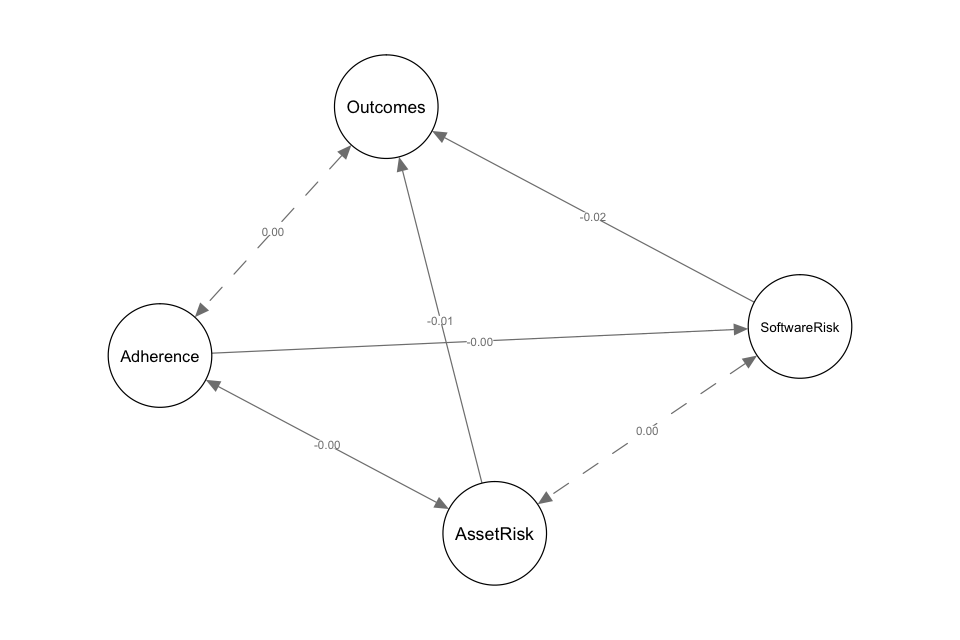
\includegraphics[width=\columnwidth]{modelzeroB.png}
	\caption{Structural and Measurement Model Overview}
	\label{fig:model_constructs}
\end{figure}

%\begin{figure}
% \includegraphics[width=\columnwidth]{modelcaoscto}
%	\caption{Model Constructs and Sub-Constructs}
%	\label{fig:model_constructs_phases}
%\end{figure}

\subsection{Measurement Model}
\label{sec:model_measurement}
%~\cite{morrison2014mapping}
%~\cite{morrison2016spefsite}
Through literature review~\cite{morrison2014mapping} and analysis~\cite{morrison2017surveying,morrison2017measuring}, we have developed a set of measurements that we expect to capture security-related factors and outcomes for software development. To collect empirical data, we have developed a data collection framework for the measurement model, available online (URL on request). In Table \ref{tab:model_spef_metrics}, we name each data element, give our hypothesis about its relationship to the structural model construct, and cite a rationale for the data element's presence. 
		
\begin{table*}[!htbp] \centering 
	\caption{Model Metrics and Hypotheses} 
	\label{tab:model_spef_metrics} 
	\begin{small}
		\begin{tabular}{@{\extracolsep{5pt}}p{3cm}p{1cm}p{2cm}p{10cm}} 
			\\[-1.8ex]\hline 
		\hline \\[-1.8ex] 
		Metric & \multicolumn{1}{c}{Effect} & \multicolumn{1}{c}{Factor} & \multicolumn{1}{c}{Rationale} \\ 
		\hline \\[-1.8ex]  
			Language	& influences &	Software Risk &   Ray et al. ~\cite{ray2014a} and Walden et al. ~\cite{walden2010idea} found small but significant effects of programming language on software quality. \\
			Operating System	& influences &	Software Risk & \\	
			Domain &	influences &	Software Risk	 & Different risks are associated with different software domains~\cite{williams2004xpef,jones2000software} \\
			Product Age	& increases &	Software Risk & Kaminsky et al.~\cite{kaminsky2011showing} and Morrison et al.~\cite{morrison2015challenges} have found evidence of code age effects on the presence of vulnerabilities. \\
			
			Source Lines of Code (SLOC)	& influences	& Software Risk & Source code size is correlated with vulnerabilities ~\cite{shin2011evaluating}, ~\cite{alhazmi2007measuring}. \\
			Churn &	increases &	Software Risk  &  Code churn is correlated with vulnerabilities ~\cite{shin2011evaluating}.\\
			Team Size	& influences	& Software Risk & Shin et al. ~\cite{shin2011evaluating} and Zimmermann et al. ~\cite{zimmerman2010searching} found correlations between team size and vulnerabilities. \\			
			\hline \\[-1.8ex] 
			Number of Machines &	increases &	Asset Risk & (Proposed) The market for machine time on botnets suggests that the number of machines a piece of software runs on increases the software's desirability to attackers. \\
			Number of Identities &	increases &	Asset Risk	 &  (Proposed) The market for personal identities and credit card information suggests that the number of identities a piece of software manages increases the software's desirability to attackers.\\
			Number of Dollars &	increases &	Asset Risk	 & (Proposed) The amount of financial resources a piece of software manages increases the software's desirability to attackers\\
			Source Code Availability	& influences &	Asset Risk & While Anderson ~\cite{anderson2002security} argues that attack and defense
			are helped equally by the open vs. closed source decision, we collect this data to enable further analysis.  \\
			Confidentiality, Integrity, Availability Requirements &	increases &	Software Risk	& Explicit security requirements for a piece of software imply a need for greater security in the software ~\cite{mell2007complete}. \\
			\hline \\[-1.8ex]
			Team Location &	influences &	Adherence	& (Proposed)  Kocaguneli ~\cite{kocaguneli2013distributed} reports on the debate over the effect of team location on software quality, collecting data on team location supports study of its effect. \\
			Methodology	& influences &	Adherence	& Different risks are associated with different software methodologies~\cite{williams2004xpef,jones2000software} \\
			Apply Data Classification Scheme & increases & 	Adherence & (Proposed) Identifying data in need of protection supports reducing Software Risk~\cite{morrison2017surveying}.\\	
			Apply Security Requirements	&	increases	&	Adherence & (Proposed)  supports reducing Software Risk[ref Riaz, etc] ~\cite{morrison2017surveying}.\\
			Perform Threat Modeling &	increases &	Adherence &(Proposed) Identification and analysis of threats supports reducing Software Risk~\cite{morrison2017surveying}. \\	
			Document Technical Stack &	increases &	Adherence & (Proposed) Understanding and controlling platform and dependency characteristics supports reducing Software Risk~\cite{morrison2017surveying}.\\	
			Apply Secure Coding Standards &	increases	& Adherence & (Proposed)  Avoiding known implementation erros supports reducing Software Risk~\cite{morrison2017surveying}.\\
			Apply Security Tooling &	increases &	Adherence & (Proposed)  Automated static and dynamic security analysis supports reducing Software Risk~\cite{morrison2017surveying}.\\
			Perform Security Testing &	increases &	Adherence & (Proposed)  Explicit validation of security requirement fulfillment supports reducing Software Risk~\cite{morrison2017surveying}.\\	
			Perform Penetration Testing &	increases &	Adherence	& (Proposed)  Exploratory testing of security properties supports reducing Software Risk~\cite{morrison2017surveying}.\\
			Perform Security Review &	increases &	Adherence	&  McIntosh et al. ~\cite{mcintosh2014the} observed lower defects for highly reviewed components. Meneely et al. ~\cite{meneely2014empirical} observed lower vulnerabilities for components with experienced reviwers. \\
			Publish Operations Guide &	increases	& Adherence & (Proposed) Documenting software security characteristics and configuration requirements supports reducing Software Risk~\cite{morrison2017surveying}.\\
			Track Vulnerabilities &	increases &	Adherence & (Proposed) Incident recognition and response supports reducing Software Risk~\cite{morrison2017surveying}.\\	
			Improve Development Process &	increases &	Adherence & (Proposed)  Adoption and adaptation of security tools and techniques based on experience supports reducing Software Risk~\cite{morrison2017surveying}.\\	
			Perform Security Training &	increases &	Adherence	& (Proposed) Development team knowledge of security risks and mitigations supports reducing Software Risk~\cite{morrison2017surveying}.\\		
			\hline \\[-1.8ex] 
			Vulnerabilities	& represent & Outcomes &  Vulnerabilities are, by definition, a negative security outcome, e.g. ~\cite{alhazmi2007measuring}.\\
			Defects & represent & Outcomes	& \\		
			\hline \\[-1.8ex] 
			\hline \\[-1.8ex] 
		\end{tabular} 
	\end{small}
\end{table*} 

\subsubsection{Software Risk}

\subsubsection{Asset Risk}

\subsubsection{Practice Adherence}

\subsubsection{Security Outcomes}


